\documentclass[12pt,a4paper]{article}

\usepackage[utf8]{inputenc}
\usepackage[T1]{fontenc}
\usepackage{lmodern}
\usepackage[margin=2.5cm]{geometry}
\usepackage{booktabs}
\usepackage{graphicx}
\usepackage{amsmath}
\usepackage{amssymb}
\usepackage{hyperref}
\usepackage{microtype}
\usepackage{setspace}
\usepackage{parskip}
\usepackage{tikz}
\usepackage{subcaption}
\usepackage{listings}

\lstset{
    basicstyle=\ttfamily\small,
    frame=single,
    numbers=left,
    numberstyle=\tiny,
    xleftmargin=2em,
    framexleftmargin=1.5em,
    language=C,
    breaklines=true
}

\hypersetup{
    hidelinks
}

\onehalfspacing

\begin{document}

\begin{titlepage}
    \centering
    \vspace*{2cm}

    {\Large\bfseries Project Checkpoint Report\par}
    \vspace{0.5cm}
    {\LARGE\bfseries Ring-Allreduce Algorithm for Distributed Gradient Synchronization\par}
    \vspace{1.5cm}

    {\large CENG342 -- Parallel Programming I\par}
    \vspace{2cm}

    {\large\bfseries Project Group 3\par}
    \vspace{1cm}

    Muhammed Fatih Asan\\[0.3cm]
    Sarper Avc{\i}\\[0.3cm]
    Mehmet Furkan Dalfidan

    \vfill

    {\large April 2026\par}
\end{titlepage}

\tableofcontents
\newpage

\section{Introduction}

Distributed model training introduces a synchronization problem. Gradients are computed on separate machines and must be aggregated. Every worker requires access to the global sum before proceeding to the next iteration. The straightforward approach designates one machine as the master, which collects all gradients, computes the sum, and broadcasts the result. This method performs adequately with two or three workers, but as more workers are added, the master node becomes a communication bottleneck.

Ring-Allreduce addresses this limitation through a decentralized approach. Workers are arranged in a ring topology where each node communicates only with its immediate neighbors. Data is partitioned into segments that circulate around the ring. In the first stage, commonly referred to as reduce-scatter, partial sums accumulate as segments traverse the ring. The second stage, allgather, distributes the completed segments to all nodes. The outcome is that every worker obtains the complete sum. The amount of data transmitted by each worker remains constant regardless of the number of workers, which constitutes the primary advantage of this approach.

The objective of this project is to implement Ring-Allreduce in C using OpenMPI. The implementation executes on a single Linux virtual machine without access to a physical cluster or GPU hardware. Instead of actual gradient tensors, float arrays initialized to 1.0 are used, which simplifies verification.

\begin{figure}[h]
\centering
\begin{subfigure}[b]{0.45\textwidth}
\centering
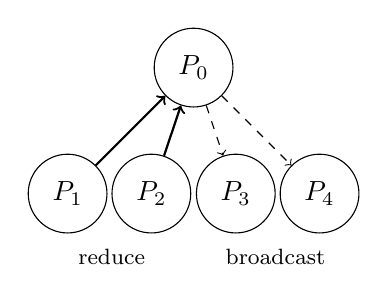
\begin{tikzpicture}[scale=0.8]
    \node[draw, circle, minimum size=1cm] (master) at (0,2) {$P_0$};
    \node[draw, circle, minimum size=1cm] (w1) at (-2,0) {$P_1$};
    \node[draw, circle, minimum size=1cm] (w2) at (-0.67,0) {$P_2$};
    \node[draw, circle, minimum size=1cm] (w3) at (0.67,0) {$P_3$};
    \node[draw, circle, minimum size=1cm] (w4) at (2,0) {$P_4$};

    \draw[->, thick] (w1) -- (master);
    \draw[->, thick] (w2) -- (master);

    \draw[->, dashed] (master) -- (w3);
    \draw[->, dashed] (master) -- (w4);

    \node at (-1.3,-1) {\footnotesize reduce};
    \node at (1.3,-1) {\footnotesize broadcast};
\end{tikzpicture}
\caption{Centralized: all traffic through $P_0$}
\label{fig:centralized}
\end{subfigure}
\hfill
\begin{subfigure}[b]{0.45\textwidth}
\centering
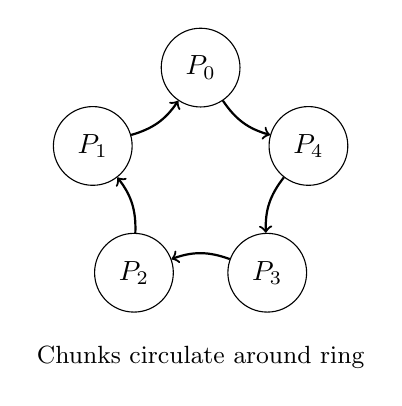
\begin{tikzpicture}[scale=0.8]
    \node[draw, circle, minimum size=1cm] (p0) at (90:1.8) {$P_0$};
    \node[draw, circle, minimum size=1cm] (p1) at (162:1.8) {$P_1$};
    \node[draw, circle, minimum size=1cm] (p2) at (234:1.8) {$P_2$};
    \node[draw, circle, minimum size=1cm] (p3) at (306:1.8) {$P_3$};
    \node[draw, circle, minimum size=1cm] (p4) at (18:1.8) {$P_4$};

    \draw[->, thick] (p0) to[bend right=20] (p4);
    \draw[->, thick] (p4) to[bend right=20] (p3);
    \draw[->, thick] (p3) to[bend right=20] (p2);
    \draw[->, thick] (p2) to[bend right=20] (p1);
    \draw[->, thick] (p1) to[bend right=20] (p0);

    \node at (0,-2.8) {\small Chunks circulate around ring};
\end{tikzpicture}
\caption{Ring: each node talks to two neighbors}
\label{fig:ring}
\end{subfigure}
\caption{Comparison of communication patterns. Left: centralized reduce-broadcast creates a bottleneck at $P_0$. Right: ring topology distributes load evenly.}
\label{fig:comparison}
\end{figure}

\newpage

\section{Related Work}

\subsection{Collective Communication in MPI}

MPI provides several collective operations, including \texttt{MPI\_Reduce}, \texttt{MPI\_Gather}, and \texttt{MPI\_Bcast}. Most MPI implementations realize these operations using tree structures or centralized root-based approaches. For small messages, tree-based algorithms perform adequately with low latency. However, for large messages, the root node becomes a bottleneck as all traffic converges at a single point.

Thakur et al.\ examined this problem in 1999 while working on MPICH. Their findings indicate that once the payload exceeds several kilobytes, tree-based collectives exhibit performance degradation. Patarasuk and Yuan subsequently provided a theoretical analysis demonstrating that ring topologies can achieve near-optimal bandwidth utilization for large messages.

\subsection{Ring-Allreduce}

Baidu's 2017 technical report brought significant attention to Ring-Allreduce outside traditional HPC circles. Their work demonstrated the algorithm's effectiveness for training models on dozens of GPUs.

The algorithm operates as follows: the array is partitioned into $n$ segments, one per worker. Subsequently, $n-1$ iterations are performed in which each node transmits its segment to the right neighbor, receives from the left neighbor, and performs element-wise addition. Upon completion, each worker holds the global sum of exactly one segment (reduce-scatter). A second loop of $n-1$ iterations follows the same communication pattern, but without summation---segments are relayed until all workers possess the complete result (allgather).

The total bytes transmitted per node is approximately $2 \cdot \frac{n-1}{n} \cdot M$, where $M$ denotes the array size. For large $n$, this expression approaches $2M$, which is independent of the number of nodes. This property constitutes the primary advantage of the algorithm.

Uber developed Horovod around this approach for TensorFlow and PyTorch. NVIDIA incorporated Ring-Allreduce into their NCCL library. Consequently, there is considerable production deployment at present.

\subsection{Profiling Tools}

For profiling MPI applications, \texttt{gprof} provides a straightforward solution. Compilation with the \texttt{-pg} flag enables instrumentation, and subsequent execution generates \texttt{gmon.out}. The output consists of a table listing function names and their respective percentages of total CPU time. Although basic, this approach addresses the fundamental question of whether execution time is dominated by MPI calls or computational routines.

Vampir and Paraver offer more sophisticated capabilities. These tools record MPI events with timestamps and provide trace visualization. Paraver was developed at the Barcelona Supercomputing Center. Both tools require additional configuration that may not be feasible within the project timeline.

\section{Methodology}

\subsection{Development Environment}

The implementation is being developed in C, with OpenMPI version 4.x for message passing. The system will execute within a Linux virtual machine on a laptop. Access to a physical cluster is not available; however, this does not compromise experimental validity. The command \texttt{mpirun -np 8 ./ring\_allreduce} will spawn eight processes on the same machine, with MPI managing communication over localhost or shared memory. This configuration will permit testing of algorithmic correctness and collection of timing measurements.

\subsection{Data Generation and Verification}

No actual training data is used. Each rank allocates a float array and initializes all elements to 1.0. With four ranks each contributing arrays of ones, the expected result after reduction is 4.0 for every element. The \texttt{verify\_results()} function performs this comparison and outputs PASS or FAIL accordingly.

\subsection{Sequential Baseline}

The baseline implementation employs the naive centralized approach. Rank 0 collects all data via \texttt{MPI\_Reduce}, computes the sum, and distributes the result via \texttt{MPI\_Bcast}. This represents the standard tree-based pattern. Timing measurements are obtained using \texttt{MPI\_Wtime()}. Five runs are performed and the median is reported to mitigate variance introduced by operating system scheduling.

\subsection{Ring-Allreduce Implementation}

The array is partitioned into $n$ chunks. When the array size is not evenly divisible by the number of ranks, the initial ranks are assigned the additional elements.

Neighbor indices are computed as follows: left neighbor is \texttt{(rank - 1 + n) \% n}, right neighbor is \texttt{(rank + 1) \% n}. Communication proceeds in the clockwise direction.

Listing 1 presents the proposed pseudocode for the reduce-scatter phase.

\begin{lstlisting}[caption={Proposed reduce-scatter pseudocode},label={lst:ring}]
left  = (rank - 1 + size) % size
right = (rank + 1) % size
for i = 0 to size-2:
    send chunk[send_idx] to right
    recv into tmp from left
    chunk[recv_idx] += tmp
\end{lstlisting}

The allgather phase will follow the same communication pattern but omit the addition operation.

Deadlock prevention is achieved through \texttt{MPI\_Sendrecv} rather than separate send and receive calls. If all ranks invoke \texttt{Send} simultaneously, no rank is available to receive, resulting in deadlock. \texttt{Sendrecv} performs both operations atomically.

Figure~\ref{fig:reducescatter} shows how data moves during reduce-scatter with four nodes. Each column is one iteration. Shaded cells indicate which chunk gets updated.

\begin{figure}[h]
\centering
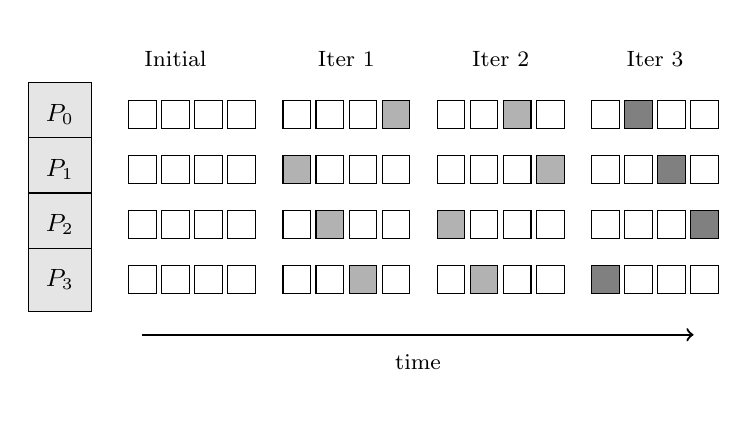
\begin{tikzpicture}[scale=0.7, every node/.style={minimum size=0.8cm}]
    \node at (0.6, 2.5) {\footnotesize Initial};
    \node at (3.7, 2.5) {\footnotesize Iter 1};
    \node at (6.5, 2.5) {\footnotesize Iter 2};
    \node at (9.3, 2.5) {\footnotesize Iter 3};

    \foreach \y/\p in {1.5/0, 0.5/1, -0.5/2, -1.5/3} {
        \node[draw, fill=gray!20] at (-1.5, \y) {\small $P_\p$};
    }

    \foreach \y in {1.5, 0.5, -0.5, -1.5} {
        \foreach \x in {0,0.6,1.2,1.8} {
            \draw (\x-0.25, \y-0.25) rectangle (\x+0.25, \y+0.25);
        }
    }

    \foreach \y/\h in {1.5/3, 0.5/0, -0.5/1, -1.5/2} {
        \foreach \x/\idx in {2.8/0, 3.4/1, 4.0/2, 4.6/3} {
            \ifnum\idx=\h
                \draw[fill=black!30] (\x-0.25, \y-0.25) rectangle (\x+0.25, \y+0.25);
            \else
                \draw (\x-0.25, \y-0.25) rectangle (\x+0.25, \y+0.25);
            \fi
        }
    }

    \foreach \y/\h in {1.5/2, 0.5/3, -0.5/0, -1.5/1} {
        \foreach \x/\idx in {5.6/0, 6.2/1, 6.8/2, 7.4/3} {
            \ifnum\idx=\h
                \draw[fill=black!30] (\x-0.25, \y-0.25) rectangle (\x+0.25, \y+0.25);
            \else
                \draw (\x-0.25, \y-0.25) rectangle (\x+0.25, \y+0.25);
            \fi
        }
    }

    \foreach \y/\h in {1.5/1, 0.5/2, -0.5/3, -1.5/0} {
        \foreach \x/\idx in {8.4/0, 9.0/1, 9.6/2, 10.2/3} {
            \ifnum\idx=\h
                \draw[fill=black!50] (\x-0.25, \y-0.25) rectangle (\x+0.25, \y+0.25);
            \else
                \draw (\x-0.25, \y-0.25) rectangle (\x+0.25, \y+0.25);
            \fi
        }
    }

    \draw[->, thick] (0, -2.5) -- (10, -2.5);
    \node at (5, -3) {\footnotesize time};
\end{tikzpicture}
\caption{Reduce-scatter phase with $n=4$. Each row is a rank, each cell is a chunk. Shaded cells are updated that iteration. After 3 iterations, each rank owns the complete sum of one chunk (dark).}
\label{fig:reducescatter}
\end{figure}

\subsection{Planned Profiling Integration}

The \texttt{-pg} flag will be added to the compiler options. Upon execution, the program generates \texttt{gmon.out}, which can be analyzed via \texttt{gprof ./ring\_allreduce gmon.out}. This indicates the distribution of execution time across functions. If 90\% of time is spent in MPI calls, communication is the dominant factor. Elevated time in helper functions may indicate optimization opportunities.

Vampir and Paraver were also evaluated. Both tools record individual MPI events with timestamps and are useful for visualizing the ring communication pattern. However, both require additional libraries and configuration. These tools may be explored if time permits after completion of the main implementation.

\section{Experimental Design}

\subsection{Parameters}

Experiments will be conducted with rank counts of 2, 4, 8, and 16. The virtual machine has 8 cores, so 16 processes will result in oversubscription; however, this should not significantly affect the validity of relative comparisons. Array sizes will range from 1\,KB to 100\,MB (24 configurations total, 5 runs each). The objective is to identify the crossover point at which the ring algorithm outperforms the baseline. Figure~\ref{fig:expected} illustrates the expected behavior.

\begin{figure}[h]
\centering
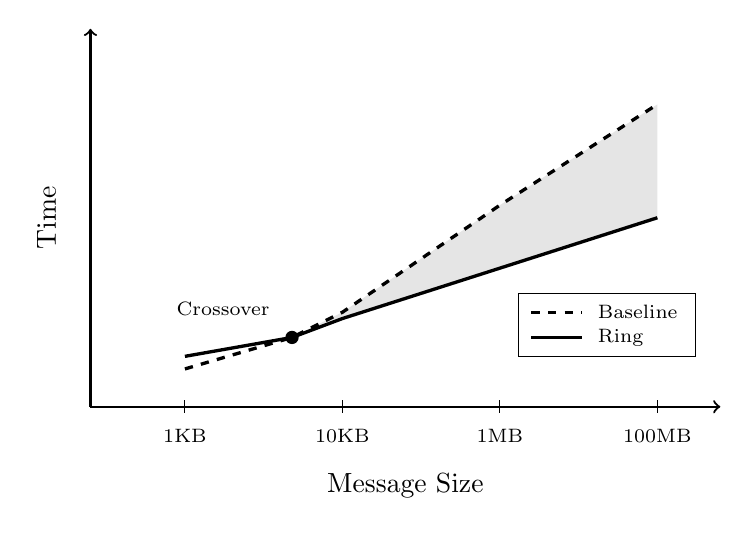
\begin{tikzpicture}[scale=0.8]
    \draw[->, thick] (0,0) -- (10,0);
    \draw[->, thick] (0,0) -- (0,6);
    \node[below] at (5,-0.9) {Message Size};
    \node[rotate=90] at (-0.7,3) {Time};

    \foreach \x/\lab in {1.5/1KB, 4/10KB, 6.5/1MB, 9/100MB} {
        \draw (\x,0.1) -- (\x,-0.1);
        \node[below] at (\x,-0.2) {\scriptsize \lab};
    }

    \fill[gray!20] (3.2,1.1) -- (4,1.5) -- (6.5,3.2) -- (9,4.8) -- (9,3.0) -- (6.5,2.2) -- (4,1.4) -- (3.2,1.1);

    \draw[line width=1.2pt, dashed] (1.5,0.6) -- (3.2,1.1) -- (4,1.5) -- (6.5,3.2) -- (9,4.8);

    \draw[line width=1.2pt] (1.5,0.8) -- (3.2,1.1) -- (4,1.4) -- (6.5,2.2) -- (9,3.0);

    \fill (3.2,1.1) circle (3pt);
    \node[above left] at (3.0,1.3) {\scriptsize Crossover};

    \draw[fill=white] (6.8,0.8) rectangle (9.6,1.8);
    \draw[line width=1.2pt, dashed] (7.0,1.5) -- (7.8,1.5);
    \node[right] at (7.9,1.5) {\scriptsize Baseline};
    \draw[line width=1.2pt] (7.0,1.1) -- (7.8,1.1);
    \node[right] at (7.9,1.1) {\scriptsize Ring};
\end{tikzpicture}
\caption{Expected performance comparison. Shaded region indicates where the ring algorithm outperforms the centralized baseline.}
\label{fig:expected}
\end{figure}

Five runs will be performed for each configuration, with the median reported. Outliers may occur due to system variability.

\subsection{Metrics}

Wall-clock time is measured using \texttt{MPI\_Wtime()}. Speedup is computed as the ratio of baseline execution time to ring algorithm execution time. A value greater than 1 indicates that the ring algorithm outperforms the baseline.

Throughput in MB/s is also recorded. Additionally, \texttt{gprof} output will be analyzed to determine which functions consume the most CPU cycles. The utility of this analysis remains to be determined, but results will be included in the final report.

\subsection{Automation}

Manual execution of 60 configurations would be impractical. A bash script, \texttt{test\_runner.sh}, will be developed to iterate over rank counts and array sizes, invoke \texttt{mpirun}, and record output to a CSV file. A separate Python script will parse the CSV and generate bar charts using Matplotlib. Although straightforward, this approach will be effective for the required analysis.

\section{Work Distribution}

The work is distributed among three team members. Member~1 is responsible for shared utilities and the baseline implementation. Member~2 implements the ring algorithm. Member~3 handles benchmarking, profiling, and report preparation. Version control follows a feature-branch workflow.

\section{Conclusion}

The project is progressing according to schedule. The algorithm has been studied and the methodology has been defined. Implementation will proceed as planned, with completion anticipated before the submission deadline.

\end{document}
